\section{Experiments} \label{sec:Experiments}
A major challenge in outlier detection research involves establishing comparability between the methods, which necessitates the implementation of a unified framework. 
Such a framework ensures that the same datasets, paradigms, and evaluation metrics are consistently applied.
The subsequent section details the practical implementation of the conducted experiments, beginning with a comprehensive analysis of the dataset. 
This examination facilitates a progressive understanding of the data, transitioning from univariate and bivariate perspectives to a structural evaluation using Uniform Manifold Approximation and Projection (UMAP). 
Following this empirical investigation, the discourse shifts to a critical assessment of potential evaluation metrics. 
These metrics are argued and justified, culminating in a definitive selection based on the previously identified data characteristics. 
The experimental framework is defined to ensure that all benchmarks maintain rigorous comparability with the InterCont methodology. 
Upon establishing this foundation, the empirical results are presented. 
To ensure statistical significance and validity, a Friedman test is employed during the evaluation process. 
Subsequently a post-hoc Wilcoxon signed-rank test is applied to rank the method' performance.
These findings are subsequently interpreted within the discussion chapter, while the final conclusions and implications of the research are synthesized in the terminal chapter of the thesis.


\subsection{Analysis of the Wine Dataset}\label{sec:data_analytics}
The Outlier Detection DataSets (ODDS) library serves as a widely utilized repository for benchmarking anomaly detection algorithms \citep{Rayana:2016}.
For instance, \citet{shenkar2022anomaly} employ these datasets to evaluate the performance of various outlier detection methods, including the previously discussed InterCont approach \citep[p. 5]{shenkar2022anomaly}. 
The repository comprises 31 distinct datasets characterized by varying dimensionalities and sample sizes. 



While utilizing a broad spectrum of datasets is advantageous for identifying the specific strengths and weaknesses of a method, analyzing all 31 datasets is beyond the scope of this thesis. 
Consequently, this research focuses on a detailed evaluation of the Wine dataset to derive insights for the results section.


The primary objective of the following analysis is to characterize the dataset's properties comprehensively. 
This process begins with a statistical summary encompassing central tendencies and distributional shape. 
This is followed by an examination of bivariate relationships between variables. 
Finally, the analysis addresses the geometric properties of the data, specifically focusing on its manifold structure.


The Wine dataset was submitted by \citet{wine_109} on June 30, 1991, to the UC Irvine Machine Learning Repository.
The original data consists of chemical analyses of wines derived from three distinct Italian cultivars. 
While initially intended for multi-class classification based on the three producers, the data was transformed into an imbalanced binary classification task for the ODDS repository.  
The processed version contains 129 instances and 13 attributes.


\begin{figure}[htbp]
    \centering
    \begin{minipage}{0.5\textwidth}
        \onehalfspacing
        In this configuration, instances from the second and third cultivars are aggregated to form the inlier class (119 instances), while 10 instances from the first cultivar are defined as outliers.  
        This results in an outlier ratio of 7.7\%, which places the dataset in comparison to other benchmarks in the repository ($mean = 8.61\%$).
        Furthermore, the version provided by the ODDS repository contains no missing values and consists exclusively of continuous variables. %\todo{good point for limitations}
        To maintain visual clarity in the subsequent analysis, feature names are omitted from certain graphical representations.
        However, Figure \ref{fig:names} provides a corresponding reference for these variable names.
    \end{minipage}
    \hfill 
    \begin{minipage}{0.45\textwidth}
        \centering
        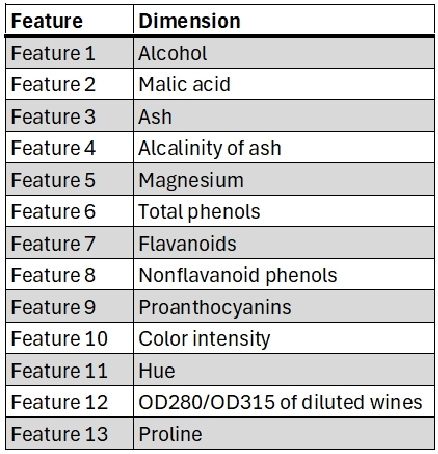
\includegraphics[width=\textwidth]{Images/Table_of_Names.pdf}
        \caption{Table of Names.}
        \label{fig:names}
    \end{minipage}
\end{figure}

\subsubsection*{Univariate Analysis}
Figure \ref{fig:boxplot} illustrates the distribution of each feature using boxplots \citep[p. 39]{tukey1977exploratory}, which display the mean, median, interquartile range ($IQR$), and whiskers defined by $1.5 \times IQR$. 
In these visualizations, the red dotted line represents the mean, while the grey line indicates the median. 


The IQR represents the central 50\% of the data points located between the $Q_1$ and $Q_3$.
A wider IQR indicates greater variability within a specific feature, whereas a narrow IQR suggests that the observations are more densely clustered. 
The features within the dataset exhibit significantly different scales of dispersion. 
While Features 3, 4, 5, and 6 are characterized by relatively narrow IQR, Feature 12 displays a notably large IQR.


The whiskers extend to most extreme data points within $Q_1 -1.5 \times IQR$ and $Q_3 + 1.5 \times IQR$ respectively, where $Q_1$ and $Q_3$ represent the first and third quartiles of the data distribution.
The relative lengths of the whiskers provide further evidence of distributional skewness. 
A top whisker that is longer than the bottom whisker indicates a right-skewed distribution, whereas the inverse suggests left-skewness. 
This asymmetry is particularly pronounced in Features 2, 6, 7, and 10, where the data distributions are notably skewed toward higher values. 
\todo{check if this comlies with the IQR}


Specific instances that exceed those thresholds represent univariate outliers.
Within this dataset, Features 3 and 4 contain three instances categorized as outliers due to their unusually low values.
Conversely, all other identified outliers across the remaining features are characterized by values that exceed the upper fence of the respective distribution.


\begin{figure}[h] 
    \centering
    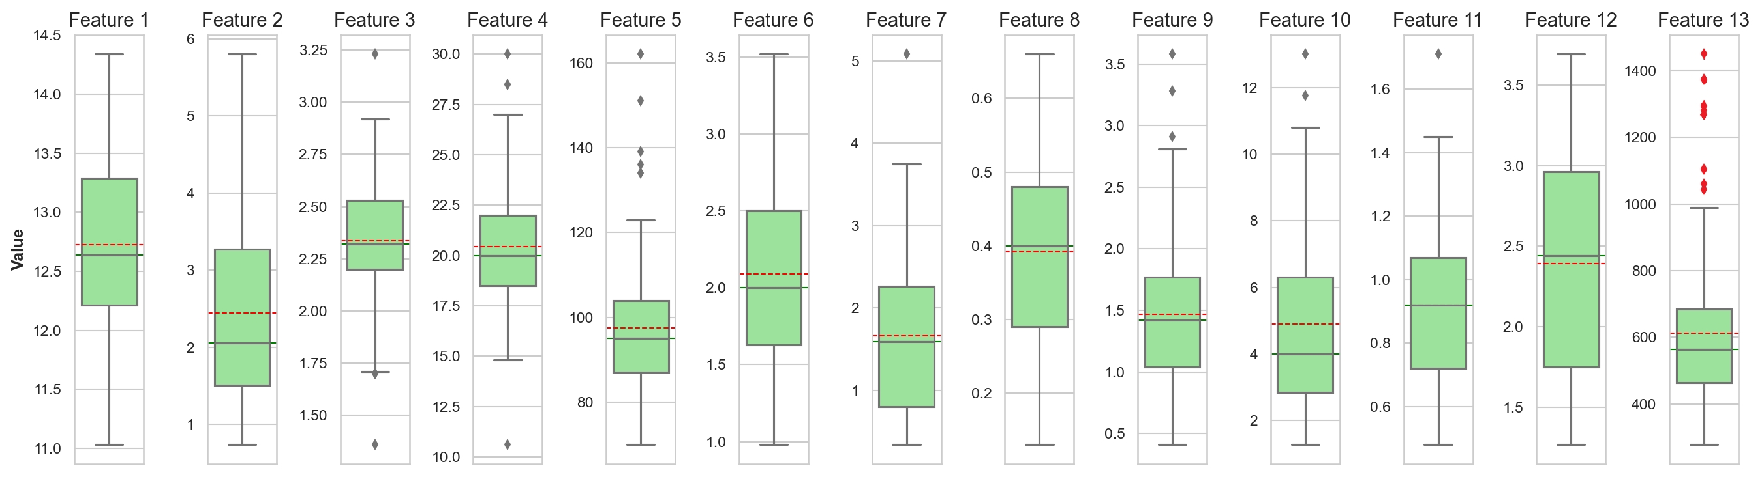
\includegraphics[width=1\linewidth]{Images/boxplots.pdf}
    \caption{Boxplots per Dimension.}
    \label{fig:boxplot}
\end{figure}
\todo{highlicht the labled outliers}


The correctly identified outliers are highlighted in red. While the boxplot analysis captures 8 out of 10 ground-truth outliers, it also yields 18 false positives. 
These eight correctly identified instances are characterized by extreme values within the Proline dimension, suggesting that the majority of the outlier class possesses an unusually high concentration of this component. 
However, such extreme values may not be inherently abnormal in a multivariate context, as their positioning could be explained by correlations with other dimensions.

To further investigate the distributional characteristics, Q-Q plots \citep{wilk1968probability} for all features are provided in the Appendix. 
Additionally, the Shapiro-Wilk test \citep[p. 592]{shapiro1965analysis} was applied to each feature. Of the 13 dimensions, only Features 2 and 3 did not show significant deviation from normality (p>0.05 and p>0.1, respectively). 
Consequently, the assumption of multivariate normality must also be rejected \citep[p. 156]{korkmaz2014mvn}.

\subsubsection*{Bivariate Analysis}
To further analyse the relationships in the dataset, a bivariate examination of the correlations between features is conducted.
In figure \ref{fig:heatmap}, the Spearman rank correlation coefficients \citep[p. 80]{Spearman1904} for all pairs of dimensions are visualized using a heatmap.
The Spearman correlation was chosen because it does not require normally distributed data, unlike the Pearson correlation \cite{Pearson1896}
Furthermore, it operates on the rank-order of values therefore the Spearman rank correlation is robust against outliers.
This metric quantifies the strength and direction of the monotonic relationship between two variables, assigning a numerical value within the range of -1 to 1.


The correlation coefficients between the dimensions exhibit significant variation. 
A positive coefficient indicates that if the values of one feature increases the value of the other increases, whereas a negative coefficient implies an inverse relationship. 
A coefficient of zero suggests that there is no monotonic relationship between the variables. 
 

\begin{figure}[h] 
    \centering
    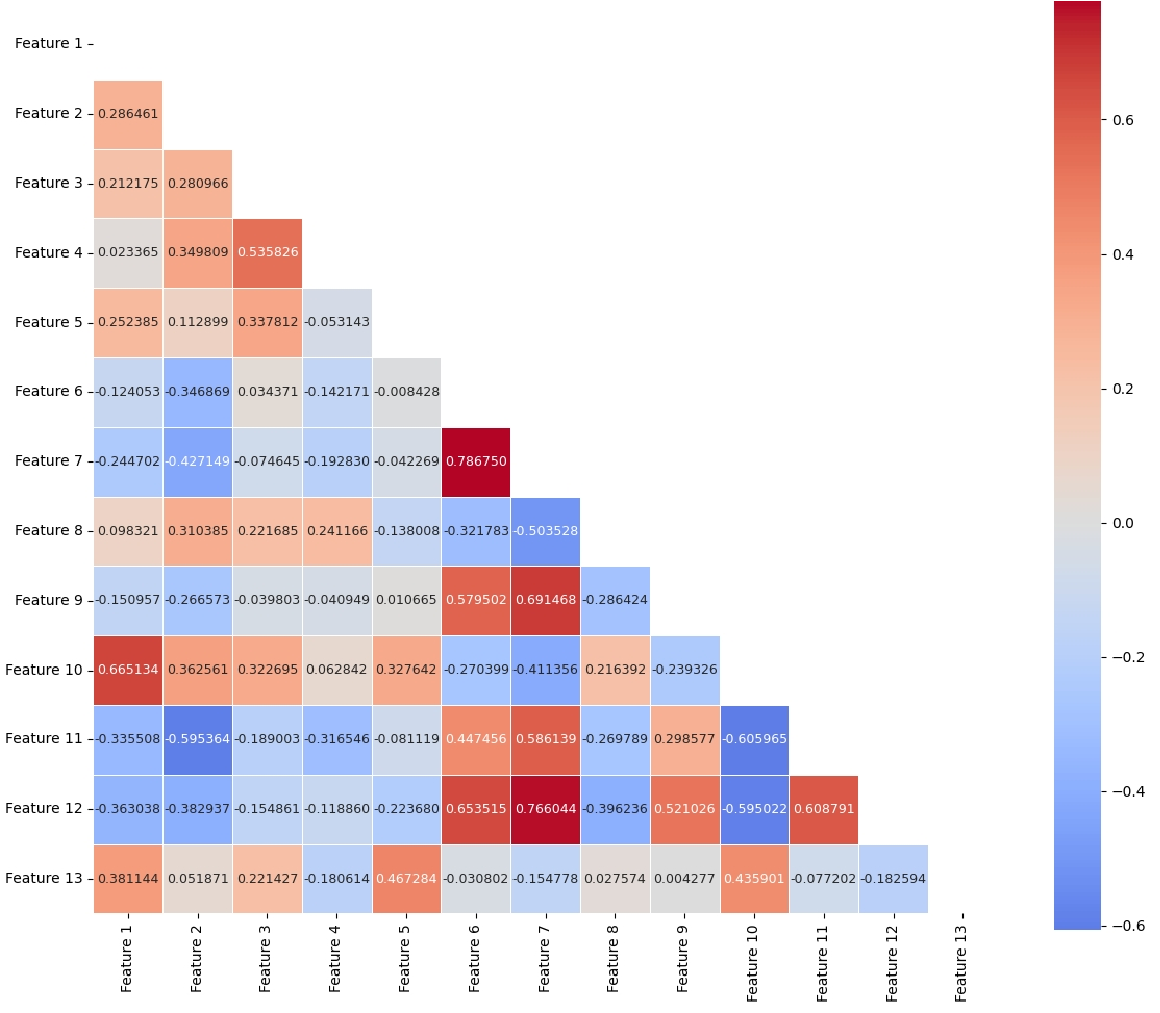
\includegraphics[width=1\linewidth]{Images/heatmap.pdf}
    \caption{Heatmap of Spearman Correlations.}
    \label{fig:heatmap}
\end{figure}


The strongest positive correlation is observed between features 6 and 7, with a coefficient of $\approx 0.79$. 
Similarly, a high positive correlation of $\approx 0.77$ exists between features 7 and  12. 
Regarding inverse relationships, feature 11 and feature 10 exhibit a strong negative correlation of $\approx -0.61$. 
The second most pronounced negative correlation, at approximately $\approx -0.60$, occurs between Features 12 and feature 10 and feature 2 and 11.
\todo{multicollinearität? MCD nicht errechenbar?}


\subsubsection*{Manifold Structure Analysis}
Analyzing the correlational structure of the dataset provides bivariate insights, yet it fails to capture the comprehensive geometric manifold of the data. 
To achieve a more profound understanding of the underlying data topology, Uniform Manifold Approximation and Projection (UMAP) \citep{mcinnes2018umap} is employed as a non-linear dimensionality reduction technique to visualize the high-dimensional observations in a lower-dimensional space. 
The subsequent section delineates the mathematical foundations of the UMAP algorithm, followed by an examination of the hyperparameters that govern the embedding process and a justification for the specific configurations selected for this study. 
Finally, the resulting visualization is presented alongside a detailed interpretation of the identified clusters and structural patterns.


The geometric manifold in the $p$-dimensional space can be highly complex globally, but locally follow a simple Euclidean structure.
The goal of UMAP is to reduce the dimensional space and to display a visualization in two-dimensional space, while preserving the global and local geometric structure.\citep{mcinnes2018umap}


UMAP requires the assumption that the data is uniformly distributed on the manifold structure, which allows it to estimate the local connectivity of the data points.
Without this assumption, the visualization would be dominated by density rather than the dataset's structure. 


UMAP constructs the low dimensional depiction in two steps:
\begin{enumerate}
    \item   Construction of the high-dimensional graph by determining the local connectivity of each instance: 
    \begin{itemize}
        \item   Estimation of distances between $x_i$ and its $k$ nearest neighbors.
        \item   Calculation of $\rho$ as the distance to the nearest neighbor. 
                By subtracting $\rho$ from all neighbor distances, UMAP ensures that every instance maintains at least one strong connection, preserving the local connectivity.
        \item   Adaptation to local density via $\sigma_i$, see equation \ref{eq:sigma}.
                Resulting in a smaller $\sigma_i$ in the locally dense regions, while a larger $\sigma_i$ in sparse regions.
        \item   Construction of a fuzzy simplicial set to merge these local views into a consistent global topological structure.
                In this context, a fuzzy simplicial set can be intuitively understood as a weighted graph where the edge strengths represent the likelihood of a topological connection between instances
    \end{itemize}
    \item   Generating the low-dimensional representation:
    \begin{itemize}
        \item   Instead of random placement, UMAP uses spectral embedding to provide a stable initial layout. 
                This captures the global topology early on and prevents the optimization from converging into poor local minima.
        \item   The algorithm iteratively adjusts the 2D positions by minimizing the fuzzy set cross-entropy.
        \item   Using Stochastic Gradient Descent, points with high connectivity are pulled together (attraction), while unconnected points are pushed apart (repulsion). 
                This continues until convergence is achieved.
    \end{itemize}
\end{enumerate}

Equation \ref{eq:sigma} describes how UMAP adapts the local connectivity and determines the parameter $\sigma_i$.

\begin{equation}
    \sum_{j=1}^{k} \exp \left( \frac{-\max(0, d(x_i, x_j) - \rho_i)}{\sigma_i} \right) = \log_2(k)
     \label{eq:sigma}
\end{equation}

Where 

\begin{equation}
    \exp \left( {-\frac{d(x_i,x_j) - \rho_i}{\sigma_i}} \right)
\end{equation}

represents the weight of the connection between instance $x_i$ and its neighbor $x_j$.
By subtracting $\rho_i$ UMAP ensures that the closest neighbor always maintains the strongest connection, as $\exp(0) = 1$.
By applying the exponential function, UMAP ensures that the influence of neighbors decreases with distance, creating a smooth decay in connectivity.
$\sigma_i$ has to be set that the sum of the exponential function over all neighbors equals $\log_2(k)$.
$\log_2(k)$ was chosen, because it ensures that the entropy of all neighbors are consistent.
A numerical optimzation process, known as binary search is applyied to find the appropriate $\sigma_i$ for each instance.


To meet this requirement, UMAP assigns in locally dense regions a smaller $\sigma_i$, which effectively stretches the space.
Conversely, in sparse regions, a larger $\sigma_i$ compresses the space.
This ensures the assumption of uniform distribution is met.


On the one hand, that depicts an outlier as an isolated instance apart from the main cluster, which coincides with the global outlier definition. 
On the other hand, the outliers is still bound to the manifold through the nearest neighbor.
Therefore the absolute distance in the diagram loses its meaning. 


When UMAP generates the low-dimensional representation, it employs a force-directed layout approach based on attraction and repulsion. 
Attraction occurs between points that exhibit strong connectivity in the high-dimensional space. 
Conversely, for instances with weak or non-existent connections, repulsion forces them apart in the two-dimensional embedding. 
These forces are adaptive to the previously calculated local affinities. 
This optimization results in a layout where clusters are grouped together even if they are sparsely distributed in the high-dimensional space, while isolated instances, often representing global outliers,are pushed away from the main data structures.


\subsubsection*{Hyperparameters}
The configuration of UMAP necessitates the specification of two primary hyperparameters that govern the construction of the low-dimensional embedding. 
Because these parameters determine the balance between preserving local and global structures, a universally optimal setting does not exist; instead, the selection depends on the specific analytical objectives. 



The first hyperparameter, $n_ {neighbors}$, defines the size of the local neighborhood considered when approximating the manifold structure. This parameter manages a trade-off between local and global features. 
A low $n_ {neighbors}$ value constrains the algorithm to focus on fine-grained patterns and intricate manifold details, which facilitates the identification of small clusters. 
Conversely, a high value incorporates a larger number of neighboring points, thereby prioritizing the broader relationships between distant regions of the data space. 
Selecting an appropriate value is essential for determining whether the data behaves as a continuous manifold or a series of discrete clusters. 


The second hyperparameter, $min_{dist}$, establishes the minimum allowed distance between points in the low-dimensional embedding. 
This parameter controls the density of the visualization by determining how compactly points are packed. 
A smaller minimum distance allows for the representation of dense clusters, whereas a larger distance forces a greater separation, emphasizing the broad topological layout over local density. 


To generate the visualization, the default hyperparameters $n_{neighbors} = 15$ and $min_{dist} = 0.1$ were utilized. 
The primary objective was to evaluate whether the Wine dataset exhibits distinct clusters or if the classes are topologically integrated. 
These standard settings provide a balanced representation that preserves both the local connectivity required for group identification and the global structure needed to observe transitions between regions. 
This configuration enables an objective assessment of the separability between the anomaly class and the inlier distribution in a two-dimensional environment. 
UMAP employs a stochastic optimization process, meaning specific coordinates may vary across different executions. 
However, iterative adjustments indicated that the underlying cluster formations remain consistent. 
Supporting evidence for this stability is provided in the appendix, where the algorithm was evaluated with $n_{\text{neighbors}} \in \{10, 20\}$ and $min_{dist} = 0.5$. 
To ensure all attributes contribute proportionally to the manifold construction, the data is normalized using the Robust transformation. 
 

The axes in the resulting UMAP plot are not directly interpretable because UMAP is a non-linear dimensionality reduction technique that projects high-dimensional data into an abstract manifold. 
In this space, the coordinates do not correspond to specific physical units or original features because the algorithm prioritizes preserving topological relationships—such as neighborhood connectivity—over the linear distances or the variance of specific dimensions. 
Consequently, while the absolute coordinates are arbitrary, the spatial proximity between points serves as a proxy for the similarity of instances in the original high-dimensional space, where smaller distances indicate greater characteristic resemblance. 


In contrast to alternative techniques, UMAP is designed to preserve a higher degree of global structure. 
Nevertheless, quantitative measurements of distances between clusters should be interpreted with caution, as the non-linear transformation into a lower-dimensional space does not maintain absolute linear distances from the original manifold.

\begin{figure}[h] 
    \centering
    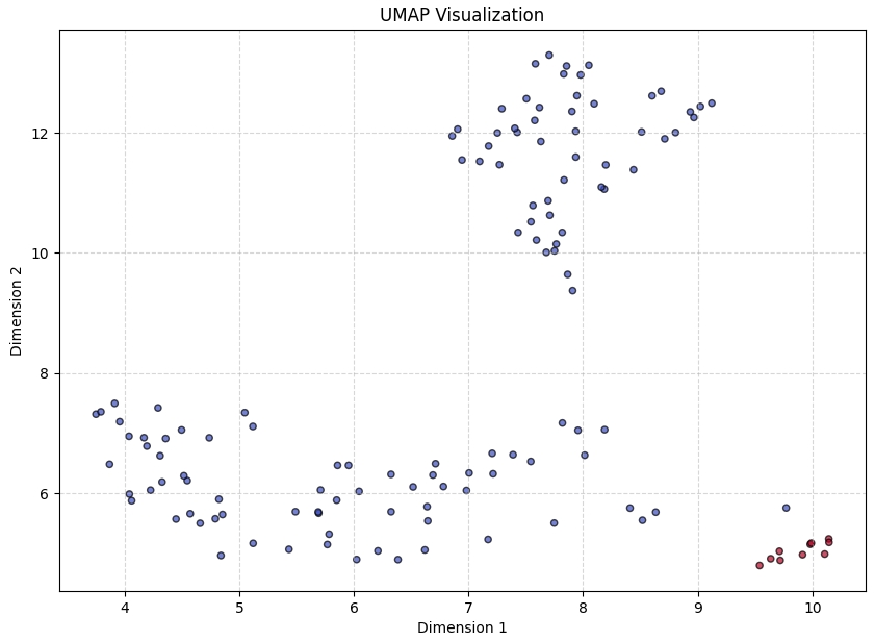
\includegraphics[width=1\linewidth]{Images/UMAP.pdf}
    \caption{UMAP of the Wine Dataset.}
    \label{fig:umap}
\end{figure}


The observations are color-coded according to their ground truth labels, with red indicating the outlier class and blue representing the inlier class.
The resulting visualization reveals three distinct topological formations and is displayed in figure \ref{fig:umap}. 


The inlier class appears as a relatively cohesive yet dispersed distribution partitioned into two primary sub-clusters, whereas the outlier class forms a highly concentrated and isolated cluster. 
Within the inlier class, the proximity of the observations suggests further distinct sub-clusters, including an elongated manifold and a dense upper-center grouping, which indicates a heterogeneous manifold for the normal data. 
Conversely, the clear spatial separation and high density of the outlier cluster, situated at the extreme right of the projection, indicate that these instances are distinct from the majority of the data. 
A single inlier observation is positioned in relative proximity to the outlier cluster, suggesting a potential boundary case or a marginal increase in similarity between the classes at that specific coordinate. 
This geometric isolation suggests that the profiles of the anomalies are significantly and consistently different from those of the inliers, which facilitates more effective detection by manifold-based and distance-based algorithms.
 

In summary the Wine dataset contains 13 dimensions from which 11 are univariatly not normally distributed, hence the multivariate distribtion is not normally distributed as well.
This violated the assumption of MCD which was discussed in chapter \ref{sec:mcd}.
The correlations of the dataset show a variety of different directions but nevertheless seems to be of linear nature.
The UMAP showed 3 distinct clusters one of which is the outlier class.
Nevertheless there are boundary cases of instances of the normal class to the outlier class.
For the distance-based method $k$-NN and may present this a serious challenge to differentiate.

